\documentclass[12pt,a4paper]{article}
\usepackage{parskip}
\usepackage[utf8]{inputenc} 
\usepackage{csquotes}
\usepackage{graphicx}
\usepackage[margin=2.54cm]{geometry}
\usepackage{fancyhdr}
\usepackage[spanish]{babel}
\usepackage[backend=biber,style=apa]{biblatex}
\DeclareLanguageMapping{spanish}{spanish-apa}
\addbibresource{bibliografia.bib}
\usepackage{microtype}
\usepackage[svgnames]{xcolor}
\usepackage{framed}
\definecolor{shadecolor}{named}{LightGray}
\pagestyle{fancy}
\fancyhf{}
\chead{Evaluacion Psicologica}
\rhead{Mateo Ardanaz}
\lhead{Universidad Católica}
\rfoot{\thepage}

\raggedright

\begin{document}

\section{Factores que afectan a los procesos de evaluacion psicologica: coordenadas de evaluacion}

Se plantea a la evaluacion psicologica como un \textbf{proceso de recogida, valoracion e integracion de informacion encaminado a tomar decisiones}. Tiene unos \textbf{propositos definidos}, desde unos supuestos sobre el \textit{comportamiento humano} y sus determinantes y desde unos \textit{supuestos metodologicos}sobre la adecuacion de las estrategias a seguir y las tecnicas a utilizar para garantizar la efectividad de la evaluacion. 

\begin{figure}[htpb]
	\centering
		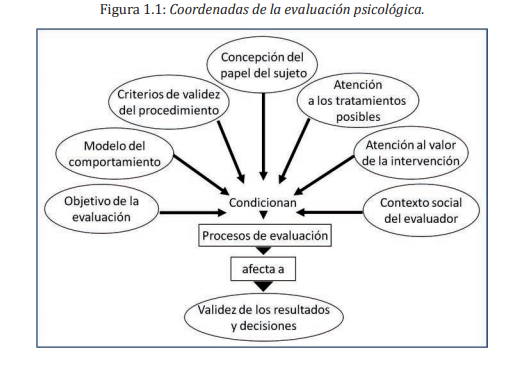
\includegraphics[width=0.8\linewidth]{coordenadas.png}
	\label{fig:coordenadas}
\end{figure}

Todos estos factores influyen en el desarrollo del proceso de evaluacion y, en consecuencia, en la validez de los resultados y decisiones que se toman en base a los mismos. 

\subsection{La concepcion del objetivo de la evaluacion condiciona el proceso y los resultados de esta}%
\label{sub:la_concepcion_del_objetivo_de_la_evaluacion_condiciona_el_proceso_y_los_resultados_de_esta}

Segun la siguiente situacion:
\begin{shaded}
\enquote{{Una de las profesoras de un centro escolar remite al psicólogo del centro un muchacho de 11 años que es bastante inquieto, a veces incluso agresivo con sus compañeros, que no presta demasiada atención en clase y cuyo rendimiento general es muy bajo. La profesora piensa si el chico debería repetir curso.}}
\end{shaded}

\pagebreak
Existen diferentes formas de afrontar este tipo de evaluacion\ldots

\begin{shaded}
{Modo 1: se examinan las calificaciones del sujeto para ver si su rendimientos es realmente bajo, luego, se examina su capacidad intelectual mediante pruebas como el \textit{WISC}, para ver si hay alguna dificultad particular. Tambien se entrevistara al profesor-padres-sujeto mismo, debido a la inquietud y a veces agresividada del niño, se buscara determinar porque se comporta asi. Dependiendo de los reslutados se realizara un informe centrado en la descripcion de las caracteristicas del sujeto.}
\end{shaded}

\begin{shaded}
{Modo 2: otra manera es observando las tareas que le pone le profesor al niño (en las que el primero afirma que el tipo se distrae y se pone violento). Se ven que tipos de conocimientos y capacidades se ponen en juego dentro del salon y como el niño hace para afrontar esas demandas en el contexto del aula. Asimismo se realizara un analisis de las caracteristicas del contexto familiar\footnote{esto se debe de hacer casi siempre me imagino} y se buscaran elementos de este que sean relevantes para el problema en cuestion. Al ver las actividades del sujeto, el investigador tratara de entender si es la naturaleza de las mismas o bien el contexto donde estas ocurren lo que dispara estas conductas indeseables en el niño.Con esos resultados el investigador podra hacer recomendaciones sobre lo mejor para el niño en estos casos.}
\end{shaded}
 
Aca se nos plantea una cosa muy curiosa. Ambos \textbf{modos de actuacion} son muy diferentes, sin embargo, ¿estan los dos bien?. 

En el primer caso tenemos mas un tipo de \textbf{indagacion en las caracteristicas del sujeto \textit{\enquote{problematico}}} cosa que permite una categorizacion de el mismo frente a otros sujetos frente a sus caracteristicas (mas o menos inteligente, mas o menos timido, etc),

La segunda por el contrario lo que intenta es un analisis de lo \textbf{vincular entre el sujeto y su contexto} y como esto puede afectar en la conducta y sentimientos del individuo.

Ambos enfoques estan bien aplicados \textbf{bajo el correcto objetivo}. Si el mismo fuera, por ejemplo, determinar si un sujeto es apto para recibir financiamiento del estado o un apoyo especial por determinada discapacidad, el primer enfoque seria adecuado. Ahora quizas ya cuando se este buscando bajo que contextos y que interacciones el sujeto logra progresar, el segundo enfoque seria el mas favorable. 

\begin{figure}[!h!]
	\centering
		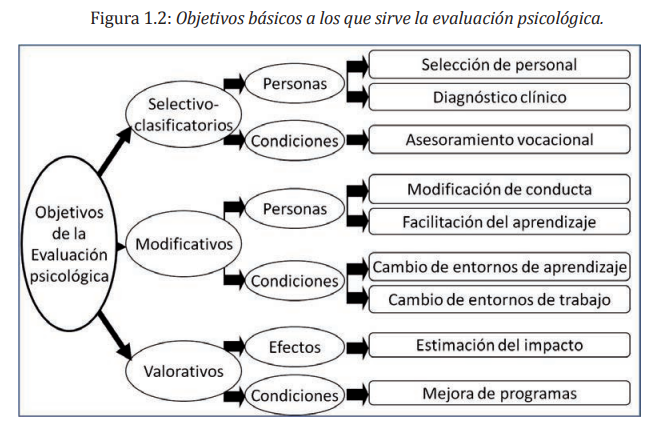
\includegraphics[width=0.6\linewidth]{objetivos.png}
	\label{fig:objetivos}
\end{figure}

Esto de que la evaluacion psicologica se realize en funcion de \textbf{diferentes objetivos} nos obliga a clasificarlos de alguna manera, para lograr ajustar las estrategias adecuadas que se deberian aplicar en cada caso. 

\subsection{Los supuestos sobre los factores que influyen en el comportamiento humano condicionan el proceso y los resultados de la evaluacion}%

Como vimos anteriormente, en los 2 casos anteriores teniamos dos supuestos. El primero buscaba la capacidad intelectual del sujeto y buscaba si su comportamiento era igual en disferentes contextos. El segundo planteaba el afecto que tiene en nuestras visiones subjetivas el ambiente y, como esto afecta nuestra conducta. 

Se plantea que no existe un modelo claro de evaluacion universalmente admitido por la psicologia contemporanea, sino modelos muy distintos (cado uno engobando incluso a posibles submodelos), que se traducen en distintos modos de proceder. Es por eso fundamental el lograr hacer una \textbf{valoracion critica} de las posibilidades y limitaciones de cada uno de ellos. 

\subsection{Los supuestos sobre la adecuacion del procedimiento a seguir y de los instrumentos a utilizar condicionan el proceso y los resultados de la evaluacion}%

Un ejemplo puede ayudarnos a entender esta mierda:

\begin{shaded}
{Un psicólogo debe seleccionar 10 sujetos para trabajar como vigilantes
jurados (Objetivo: seleccionar). Entre otras cualidades considera que los candidatos deben poseer un elevado nivel de asertividad, dado que deben ser
capaces de ser firmes y hacer respetar las normas sin ser agresivos (Parte
de una conceptualización de las cualidades como rasgos). Para evaluar estas
cualidades decide utilizar una de las escalas de asertividad existentes en el
mercado. El problema con el que se enfrenta entonces es el de decidir cuál de
ellas utilizar pues, dependiendo de la elección, el resultado final del proceso
de selección de personal puede ser más o menos adecuado.

¿Debe aceptar cualquier escala que diga medir asertividad? ¿Debe analizar el contenido de los elementos? ¿Debe buscar en el manual de la prueba
información sobre el grado en que las cualidades medidas se manifiestan de
modo regular y estable en el tiempo? ¿Debe buscar información sobre el grado en que las puntuaciones en la prueba permiten anticipar el modo en que
los sujetos tienden a actuar en situaciones reales? ¿Qué debe hacer si no encuentra alguno de los datos de información referidos?}
\end{shaded}
 
Cuando hablamos de \textbf{validez} de un test, hablamos de el grado de exactitud con el que este mide el contructo teorico que pretende medir, y si se puede utilizar con el fin previsto. 

En el caso de que, por ejemplo, quiera estudiar el nivel de aprendizajes adquiridos en estudiantes de ingenieria a lo largo de su primer año, no puedo utilziar un test que mide el nivel de aprendizaje adquirido pero que se creo para la utilizacion en un contexto de estudiantes de psicologia en su año de graduacion. 

Lo mismo en el caso de querer aplicar un test de rendimiento escolar en niños de la mejor escuela del pais, cuando el test fue creado para una poblacion de estudiantes de escuelas publicas. 

\subsection{La concepcion del psicologo acerca del papel del sujeto o sujetos evaluados durante el proceso de evaluacion condiciona el proceso y los resultados de esta}%

Cuando una persona pide ayuda a un psicologo para resolver un problema, este comienza a recoger informacion guiado por sus ideas sobre la naturaleza del problema a abordar, por los objetivos a conseguir, etc. El problema aca es que muchas veces se pierde de vista que el sujeto \textbf{no es unicamente pasivo, sino activo}. El paciente esta continuamente haciendo inferencias de la utilidad de lo que le estan haciendo hacer, se cuestiona todo, y muchas veces si no se tiene en cuenta esta dimension, puede ocurrir el classic abandono del tratamiento. 

Un claro ejemplo de esto seria que empezaramos el \textit{WAIS} o el \textit{WISC} desde la pregunta mas dificil hasta las mas facil. ¿Que pasaria por la mente del sujeto si se lo expone a constantes fracasos los primeros reactivos?. Claramente la frustracion para algunas pesonas seria elevadisima, y en test largos como estos dos podria llevar a un abandono o a una baja de motividad tremenda. 

En resumen hay que tener en cuenta que la persona que esta del otro lado de la evaluacion es tambien una puta persona. Gracias capitan obvio. 

\subsection{La atencion a los tipos de intervencion disponibles entre los cuales es preciso escoger condiciona la organizacion y efectividad del proceso de evaluacion}%

Cuando recogemos informacion con el objetivo de poder ayudar a las personas a cambiar, es fundamental que la informacion no sirva solo para definir el problema, sino tambien para \textbf{decidir como intervenir}.  

Ciertamente la \textbf{eficacia} de el tratamiento, es lo que va a permitir la mejora del sujeto y en ocasiones la desaparicion de los problemas del sujeto. 

Es importante diagnosticar diferentes tratamientos a pacientes que presenten la misma patologia, asi por comparacion podemos saber cual es la mas eficaz para el problema.

\subsection{La importancia que se concede a la valoracion de los efectos de la intervencion condiciona el proceso y los resultados de la evaluacion}%

Basicamente se explica que luego de un proceso de intervencion, debe existir un proceso valorativo, donde se conteste si se contestaron los objetivos, que efectos ha tenido la intervencion en el sujeto, a que se le atribuye la falta de logros, etc. 

Para esto necesitamos un adecuado \textbf{diseño de un proceso de valoracion}. 

\subsection{El contexto en el que se realiza la evaluacion influye en el planteamiento, desarrollo y uso de los resultados de la misma}%

Un ejemplo claro. Muchos profesores piensan que el problema no son ellos, sino los alumnos. Esperan a que estos sean evaluados fuera de el salon de clases a ver si le pueden seguir el ritmo a los demas. Si el psicologo responde a estas expectativas y evalua el problema centrandose en el sujeto, su tarea puede ser infeicaz, pues los resultados de la evaluacion no le permitirian actuar sobre las variables que estan determinando el problema en si.

\section{Aplicacion de test psicologicos}%

\begin{shaded}
El termino \textit{\enquote{test}} nace con \textbf{McKeen}, que explica que los test mentales eran \textbf{sistemas normalizados de procedimientos} que permitian obtener informacion \textbf{objetiva} respecto al rendimiento de las personas en la realizacion de tareas tipo. 
\end{shaded}

Aunque las definiciones de testi psicologicos formuladas han sido diversas, todas ellas coinciden en algunos aspectos comunes\ldots

\begin{shaded}
\textbf{Anastasi} plantea que un test que un test psicologico es escencialmente \textbf{una medida objetiva y estandarizada de una muestra de conducta}.  
\end{shaded}

Cuando hablamos de \textbf{uniformidad}, hablamos de una uniformidad en el procedimiento de administracion y puntuacion del test; es decir, el test sera administrado en una situacion controlada y la puntuacion obtenida sera interpretada comparandola con la de un grupo normativo. 

El otro elemento interesante de la definicion es el \textbf{ \textit{\enquote{muestra de conducta}}}. Es decir, lo que se evalua con un test psicologico no es mas que una muestra de conductas, por lo que la efectividad del mismo radica en la correcta eleccion de los items que representan al conjunto total de conductas que queremos evaluar. 

\begin{shaded}
\textbf{Cronbach} define al test psicologico como \textit{\enquote{un procedimiento sistematico para observar la conducta y describirla con ayuda de escalas numericas o categoricas establecidas}}.
\end{shaded}

En esta definicion vemos mas presente el aspecto estadistico y matematico de los test.

Un test psicologico por tanto es un instrumento de medida que debe cumplir las siguientes caracteristicas:

\begin{enumerate}
	\item Es una \textbf{muestra de conductas}: solamente se incluye un posible grupo de conductas que permiten evaluar algun atributo (la extroversion) o predecir algun resultado (exito en determinado puesto de trabajo, profesion). 
	
	\item La muestra de conductas es obtenida bajo \textbf{condiciones estandarizadas}: el test siempre se presenta en el mismo orden, de la misma manera, con los mismos estimulos y las mismas instrucciones. Los procedimientos de puntuacion tambien son sumamente consistentes. 

	\item \textbf{Establece una puntuacion}: el test psicologico proporciona informacion cuantitativa acerca de la conducta; ademas sus resultados son puramente objetivos y comprobables por cualquiera. 

	(\textbf{Murphy y Davidshofer - Rogers})
\end{enumerate}

Hay tipos de test que no cumplen con el requisito de objetividad, tales son los \textbf{test proyectivos}. De ahi que utilizen comunmente el termino \textit{\enquote{tecnica}}, para lograr establecer una diferenciacion. 

\section{Psicodiagnostico}

Desde que \textbf{Rorschach} lo trajo al habla, se ha entendido como psicodiagnostico a \textbf{las tecnicas proyectivas y al modelo medico de evaluacion psicologica}. 

Las asignaturas de psicodiagnostico, que en un principio se correspondian en gran parta a tecnicas proyectivas, fueron integrando las distintas innovaciones, tanto en tecnicas como en modelos, sin modificar los nombres de las asignaturas. 

En un estudio realizado en los 80 por \textbf{Blanco y leon} se establece que el concepto de psicodiagnostico tiene una doble vertiente. Por un lado se refiera a la exploracion psicologica a traves de los test, y por otra, a la evaluacion y el analisis cientifico del comportamiento. 

\section{Evaluacion psicologica}

Aparece por primera vez en el 48. Se plante que en la evaluacion psicologica se tienen en cuenta los \textbf{aspectos positivos} de la persona, a diferencia de el conocido psicodiagnostico, donde solo se veia la patologia. 

Se utilizo mucho durante la 2GM para ver a quienes podian y a quienes no podian mandar a la guerra. 

\begin{shaded}
\textbf{Maloney y Ward (1976)} establecen a la evaluacion psicologica como \textit{\enquote{un proceso variabe de solucion de problemas que utiliza diferentes procedimientos de recogida de datos}}.
\end{shaded}

Segun estos la evaluacion tiene 3 partes importantisimas:

\begin{enumerate}
	\item El planteamiento de un problema.
	\item La recogida de datos.
	\item Interpretacion de estos datos y la solucion. 
\end{enumerate}


La evaluacion psicologica incluye \textbf{muchos paradigmas de evaluacion}, tales como la evaluacion conductual y la de personalidad; muchos \textbf{metodos de evaluacion}, como la observacion directa y los cuestionarios de autoinforme; y muchos \textbf{instrumentos de evaluacion}, como cuestionarios de autoinforme para la depresion, protocolos de evaluacion psicofisiologica para trasntornos de PTSD o metodos de observacion de conductas de padres e hijos para uso clinico.

Asi como son diversos en esto tambien lo son en sus objetivos. 

\section{Valoracion}%

\begin{shaded}
	Segun \textbf{Fernandez Ballesteros (1985)} la valoracion hace referencia a la \textit{\enquote{estimacion de las cualidades de un concreto tratamiento, intervencion o programa que es aplicado en un contexto determinado, a unos concretos individuos y con unas repercusiones conductuales especificas}}.	
\end{shaded}

Hoy en dia la sinonimia entre los conceptos de evaluacion y valoracion provocan que se utilize evaluacion para entender lo que abarca tambien la valoracion. 

\section{El proceso como procedimiento cientifico y sus variables}%

La evaluacion psicologica implica un proceso, es decir, conlleva una serie de pasos que han de producirse en un cierto orden.

Las dos principales caracteristicas del proceso de evaluacion son:

\begin{enumerate}
	\item Que implica un proceso de \textbf{toma de decisiones} para llegar a la solucion de un problema evaluativo.
	\item Que requiere la \textbf{formulacion y contrastacion de hipotesis}.
\end{enumerate}

El proceso de evaluacion comienza cunado el cliente o un relativo del cliente realiza una demanda a un profesional de la psicologia. A partir de ese momento se inicia un proceso para resolver la cuestion planteada. Necesariamente para resolver esto, se deberan tomar decisiones a traves de una serie de fases o momentos que, en terminos generales, son los mismos que los utilizados en la investigacion de cualquier tipo de conocimiento cientifico y, por tanto, se pueden considerar un proceso de \textbf{formulacion y contratacion de hipotesis}. 

Hoy en dia la evaluacion responde a muchos problemas y objetivos (diagnostico, orientacion, seleccion, tratamiendo, cambio, etc), pero anteriormente no era asi. En un principio la evaluacion psicologica estaba casi ligada al ambito clinico y, por tanto, tenia una sola meta: la del diagnostico. Se buscaba asignar una categoria en un sistema de clasificacion psiquiatrico a un sujeto determinado.  

Por otra parte, la orientacion o consejo psicologico es aquella meta de la evaluacion por la cual el estudio psicologico del sujeto se realiza con el fin de dar ayuda a la hora de tomar decisiones o establecer planes de accion referidos a un futuro (eleccion vocacional). El terapeuta debera tener en cuenta las aptitudes y virtudes del sujeto, sus preferencias vocacionales, etc. 

La evaluacion puede tener objetivos de seleccion en el caso de que la demanda sea una seleccion de personal.

Por ultimo la evaluacion puede realizarse con objetivos de tratamiento y cambio del comportamiento del sujeto como objeto de estudio. En otras palabras requeririamos una evaluacion del sujeto ya que hay un deseo de intervenir en la persona para producir cambios positivos en su conducta. 

\begin{shaded}
	Aunque la evaluación en todos los casos se lleve a cabo a partir de un modelo teórico (el formulado en el capítulo anterior) y una base de conocimiento específica (la del problema que se
presenta), no cabe duda de que existirán matices
diferenciales según se trate de diagnosticar, orientar, seleccionar o tratar para producir un cambio.
En efecto, mientras que los objetivos científicos
de esas tres primeras metas podrían reducirse a
unas operaciones básicas como son las de clasificar, describir y predecir la conducta, el tratamiento y cambio requieren una explicación del comportamiento objeto de estudio. De ello se deduce
que objetivos de evaluación diferentes requieran procedimientos de actuación diferentes. Así,
mientras que el diagnóstico, la orientación y la
selección exigen la predicción del comportamiento y se pueden realizar mediante planteamientos
metodológicos observacionales y correlacionales,
no sucede así a la hora de proceder al cambio de
conducta, que, a su vez, requiere la planificación,
administración y valoración de intervenciones; en
este caso se exigen métodos experimentales o cuasiexperimentales.
\end{shaded}


\section{El proceso descriptivo-predictivo}%

\begin{figure}[!h!]
	\centering
	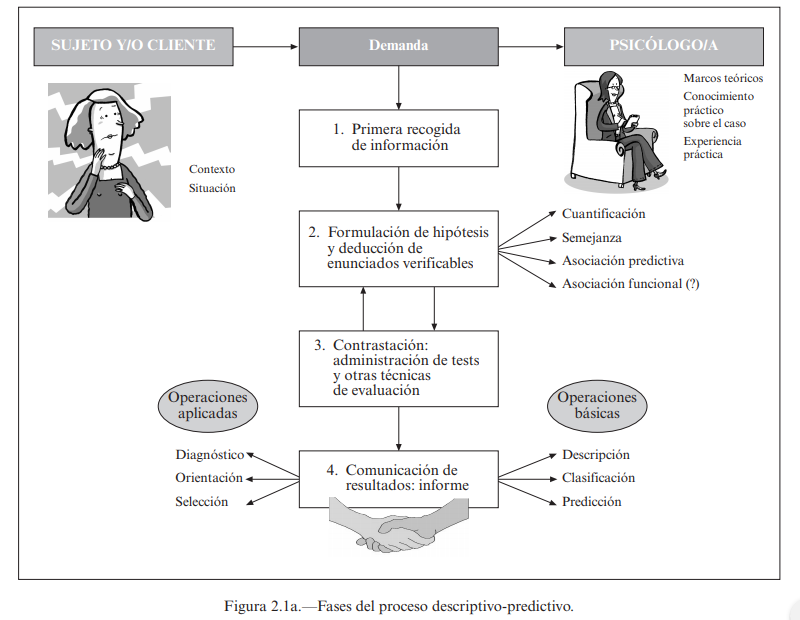
\includegraphics[width=1\linewidth]{fases.png}
	\label{fig:fases}
\end{figure}

\subsection{Fase 1: primera recogida de informacion}

En un principio el evaluador se situa como \textbf{observador participante}. Es como un recolector de informacion. 

Durante esta fase es impresindible recaudar datos suficientes sobre las siguientes cosas:

\begin{enumerate}
	\item Especificar la demanda y fijar objetivos sobre el caso.
	\item Establecer las condiciones historicas y actuales que vengan al caso (basicamente el contexto social, ambiental y el historial medico/clinico de la persona y de su familia).
\end{enumerate}

\subsubsection{Especificar la demanda y fijar objetivos sobre el caso}%

La demanda puede ser o bien planteada por el sujeto mismo o por un tercero, que se convierte en cliente de la evaluacion (juez, medico, padres, etc). 

La idea de aclarar los objetivos es fundamental. Muchas veces sucede que el sujeto no tenga muy clara su demanda y, por tanto, no tenga idea cuales son los objetivos que quiere plantear. Ahi el terapeuta debe ayudarlo en la trasnformacion de planteos posiblemente vagos a terminos concretos. 

Una breve guia de esto:

\begin{itemize}
	\item Motivo de consulta.
	\item Porque solicita la evaluacion.
	\item Que se desa conseguir de esta.
	\item Cual es la demanda concreta en terminso de diagnostico, orientacion, seleccion o tratamiento y cambio.
	\item Y, en su caso, cuales son los comportamientos que, inicialmente, van a construir el objeto de analisis en este caso concreto. 
\end{itemize}

Esta primera entrevista debe de realizarse con tecnicas de amplio espectro\footnote{creo que se refiere a una entrevista abierta, o semi-estructurada con preguntas que dejen que el sujeto se explaye.}. 

Se plantean 2 cuestiones eticas importantes que el terapeuta debera tener en cuenta:

\begin{enumerate}
	\item Si se trata de una demanda licita (legal).
	\item Si el psicologo esta capacitado para abordar la demanda y cumplir los objetivos. 
\end{enumerate}


Una vez que el psicologo acepta, debe informar:

\begin{itemize}
	\item Que va a ser administrada una serie de técnicas, tests y otros instrumentos psicológicos, para lo cual solicita su conformidad.
	\item Que todos ellos requerirán de su colaboración.
	\item  Que toda la información que se obtenga se mantendrá en la misma estricta confidencialidad.
\end{itemize}

Si esto es aceptado por el cliente tamos chetos

\subsubsection{Especificar las condiciones historicas y actuales potencialmente relevantes al caso}%

Es necesario indagar en los aspectos ambientales y personales que forman parte de la historia del sujeto. Lo que nos interese de esa historia claramente va a depender de la demanda planteada al principio. 

En cuanto a datos historicos:
\begin{itemize}
	\item Calificaciones escolares.
	\item Examenes medicos.
	\item Etc\ldots
\end{itemize}

En cuanto a datos actuales:
\begin{itemize}
	\item Habitat (donde vive, con quienes, etc).
	\item Condiciones familiares, sociales y economicas.
	\item Eventos vitales actuales.
	\item Ocupacion.
	\item Ocio y tiempo libre.
	\item Estilio de vida.
	\item Estado fisico y de salud.
	\item Valores.
	\item Otras condiciones potencial relevantes al caso. 
\end{itemize}

\subsection{Fase 2: formulacion de hipotesis y deduccion de los enunciados verificables}%

Esta fase se realiza en funcion de las observaciones e informaciones obtenidas, si estas ultimas son de mala calidad, las hipotesis probablemente tambien lo sean. 

\subsubsection{Formulacion de hipotesis}%

Aca realizamos un analisis de la informacion obtenida y debemos preguntarnos lo siguiente:

\begin{itemize}
	\item Que tan fiables son los datos que obtuvimos?
	\item Que tanto conocimiento tenemos nosotros para realizar las conexiones necesarias entre estos datos para llegar a un planteo hipotetico.
\end{itemize}

Hay 4 tipos de supuestos:

\begin{enumerate}
	\item Supuestos de \textbf{cuantificacion}: se trata de comrobar que un determinado fenomeno se da y en que medida aparece segun ciertos parametro.
	
	\item Supuestos de \textbf{semejanza}: se trata de poner al sujeto dentro de una categoria que se encuentre en algun sistema de clasificacion. 

	\item Supuestos de \textbf{asociacion predictiva}: se trata de hipotetizar en que medad las conductas del objeto de estudio se dan asociadas a otras (la falta de rendimiento escolar del niñoesta asociada a comportamientos hiperactivos - sujeto presenta aptitudes que lo harian un gran estudiante de ingenieria).

	\item Supuestos de \textbf{asociacion funcional}:????????????? 
\end{enumerate}

En resumen...

\begin{shaded}
Diagnostico $\rightarrow$ cuantificacion y semejanza.

Orientacion/seleccion $\rightarrow$ cuantificacion y asociacion predictiva.

Cambio comportamental $\rightarrow$ relacion funcional o causal que verificaremos mediante pruebas observacionales o correlacionales.
\end{shaded}

\subsubsection{Deduccion de enunciados verificables}%

Tenemos que:

\begin{itemize}
	\item Realizar el listado de las variables implicadas.
	\item Seleccionar los test y tecnicas correctas (usando criterios psicometricos).
\end{itemize}

Se busca que cada una de las variables este operacionalizada por mas de un instrumento, para conseguir la debida triangulacion. Esto es fundamental, porque por la naturaleza de los constructos estudiados en la psicologia, es muy raro que existan \textit{\enquote{medidas verdaderas}}. 

\subsection{Fase 3: contrastacion; administracion de test y otras tecnicas de evaluacion}%

Esto tiene tres subfases:

\begin{enumerate}
	\item Preparacion y planificacion de los instrumentos a utulizar.
	\item Administracion de los test y tecnicas seleccionadas a traves de los procedimientos establecidos. 
	\item El analisis de los resultados en orden a la comprobacion de las hipotesis (si no se contrastan se plantean nuevas hipotesis).
\end{enumerate}

\subsection{Fase 4: comunicacion de los resultados (el informe)}%

Todo proceso de evaluacion concluye con la integracion de todos los resultados obtenidos y su comunicacion al cliente-sujeto. Esto es una conducion cientifica, asi como un requisito etico. 

\subsubsection{Integracion de los resultados}%

Basicamente esto es la formulacion del informe. Dependera de cada caso particular, y depende tambien de los datos obtenidos si llegamos a una mera descripcion o clasificaion del sujeto o si logremos realizar predicciones sobre la conducta del mismo. Dependera tambien de esto ultimo si corresponda hacer alguna recomendacion de intervencion. 

Las cosas que obtengamos que transciendan la demanda o los objetivos de la evaluacion, deberan ser integradas en los resultados y en el caso que no sea pernitente que se escriba (madre abusada se le comenta a la institucion) deberan omitirse pero ser comunicadas en la parte oral.??

\subsubsection{Comunicacion de resultados: el informe oral y/o escrito}%

Esto se explica solo.

\section{El proceso interventivo-valorativo}%

\begin{figure}[!h!]
	\centering
	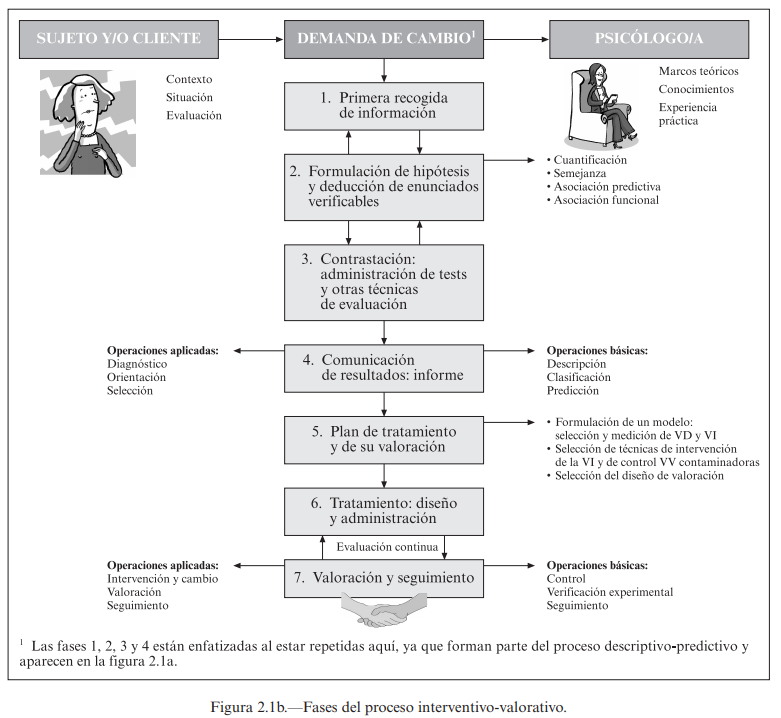
\includegraphics[width=0.8\linewidth]{fases1.png}
	\label{fig:fases1}
\end{figure}

Cuando la demanda o los objetivos del cliente son de cambio o modificacion del comportamiento(cosa que tambien requiere una explicacion de la conducta a cambiar o modificar), el evaluador tiene que adoptar esta variante del proceso en la que a la hora de comprobar las hipotesis, se exige una intervencion y su valoracion.

En su primera parte podemos decir que es identico al descriptivo-predictivo, ya que en todo proceso de evaluacion interventivo tiene que hacer una previa formulacion empirica del caso (realizada normalmente a partir de metodologias observacionales y correlacionales).

Es a partir de ahi que el evaluador se planteara unas hipotesis explicativas que va a terminar verificando, esta vez, a traves de la manipulacion experimental, mediante un determinado tratamiento. 

Basicamente tenemos el clasico experimento con variables dependientes y variables independientes. 

\subsection{Fase 5: plan de tratamiento y su valoracion}%

Una vez que concluimos el descriptivo-predictivo, tecnicamnte tendriamos que saber no solo cual es el problema sino cuales son las condiciones que hipoteticamente lo causan o mantienen. 

Por tanto habremos generado \textbf{hipotesis funcionales} que constituyen la teoria sobre el caso.

En resumen, ya tendriamos que saber cuales son las variables dependinetes que pretendemos modificar y cuales son las variables causales o independientes que son las que mantienen/provocan el problema en cuestion.

\subsubsection{Teoria sobre el caso}%

\textbf{Seleccion de las variables dependientes e independientes}: el establecimiento de una teoría sobre el caso está implícito en cualquier intervención, sea cual fuere el marco teórico de partida. Se aplica un tratamiento porque se supone que el problema objeto de estudio está «causado», controlado, mantenido o relacionado funcionalmente con una determinada variable relevante. Es esta variable (independiente) la que manipularemos con nuestro tratamiento.

\textbf{Seleccion de las medidas de las variables dependientes e independientes}: 




\end{document}
